\chapter{Continual Learning}
\label{ch:06-continual-learning}

\lecturemeta{Clare Lyle}{Google DeepMind}

Lyle's framing is that continual learning is two problems, not one, and that standard
training is bad at both. A network must remember what it learned before, and it must remain
able to learn something new. The first failure is catastrophic forgetting and has been known
since the early 1990s; the second is loss of plasticity and is the subject of most of the
lecture, because it is both less obvious and better understood mechanistically. The line that
organises everything is slide 17, which reads: ``Continual learning doesn't have to be hard
(unless you want to use a neural network)''. The difficulties are properties of the optimiser and the
architecture, not of the problem statement, and once diagnosed that way most of them have
mundane fixes.

\section*{Key ideas}

\paragraph{Two problems and a meta-problem.} Problem one is remembering the
past~\citep{kirkpatrick2017}. Problem two is retaining plasticity, the capacity to keep
learning at all. The meta-problem is evaluation, and neither option is satisfactory: train on a pre-specified sequence of tasks, which is artificial, or find an
application that is naturally continual, which is uncontrolled. That tension sits under every result in the field.

\begin{figure}[htbp]
\centering
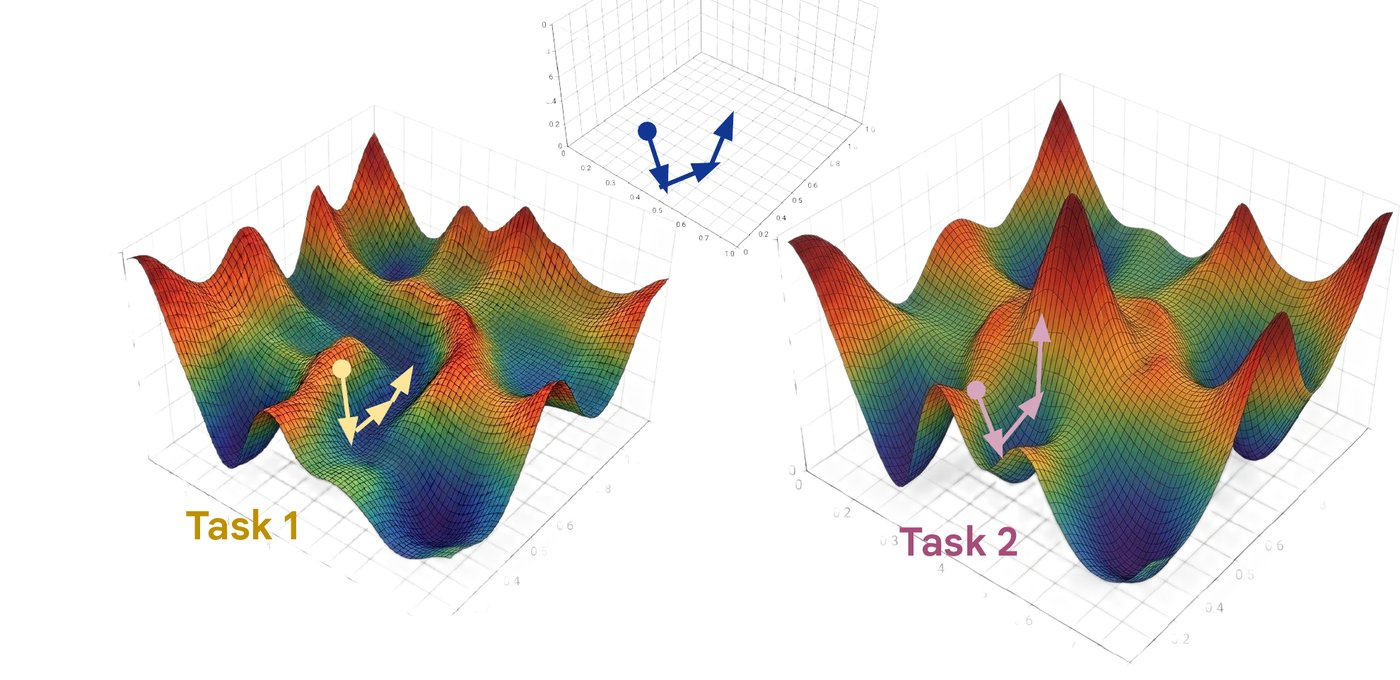
\includegraphics[width=0.88\textwidth]{figures/continual-learning-2.jpg}
\caption{The geometric intuition for catastrophic forgetting, from the Continual Learning
lecture. The same parameters sit on two different loss surfaces, one per task, and the descent
directions the two tasks ask for are not aligned, as the inset axes make explicit. A step that
lowers the task-two loss can climb the task-one loss, so progress on the new task is paid for
out of the old one.}
\label{fig:continual-learning-2}
\end{figure}

\paragraph{Forgetting is gradient conflict, and the fixes follow from that.} The intuition given is geometric
(Figure~\ref{fig:continual-learning-2}): gradients on different tasks often conflict, so a step
that helps task two moves parameters out of the region that solved task one. Three families of solution follow
directly from the diagnosis, and the lecture states them in plain terms before naming any
method. Do not change the parameters used for the old task too much, which is regularisation
and, with a different mechanism, sparsity and network expansion. Keep the old data around and
keep training on it, which is replay. Or periodically reset the model and retrain on
everything, which pairs with distillation. Lyle's practical verdict appears again in the summary: if the data can be kept, the first problem is easy. Only under a memory constraint
does it require finesse.

\paragraph{Loss of plasticity has a mechanism, and it is the optimiser.} Under repeated task
changes networks become less trainable over time, in the extreme case with dead
ReLUs and a model emitting a uniform distribution. Two causes are separated. First, gradual
convergence toward bad parameters, diagnosed through the empirical NTK matrix at convergence.
Second, and more surprising, destructive updates that happen almost immediately after a task
change. The reason is that optimisers are built for stationary problems. In Adam the second
moment estimate decays slowly, with the usual 0.99, so it reflects the small gradients seen at
the end of the previous task; when the loss changes the numerator grows at once while the
denominator lags, and the effective step size becomes enormous
(Figure~\ref{fig:continual-learning-1}). The loss landscape has meanwhile evolved to be stable
only at the small step size it was trained with.

\begin{figure}[htbp]
\centering
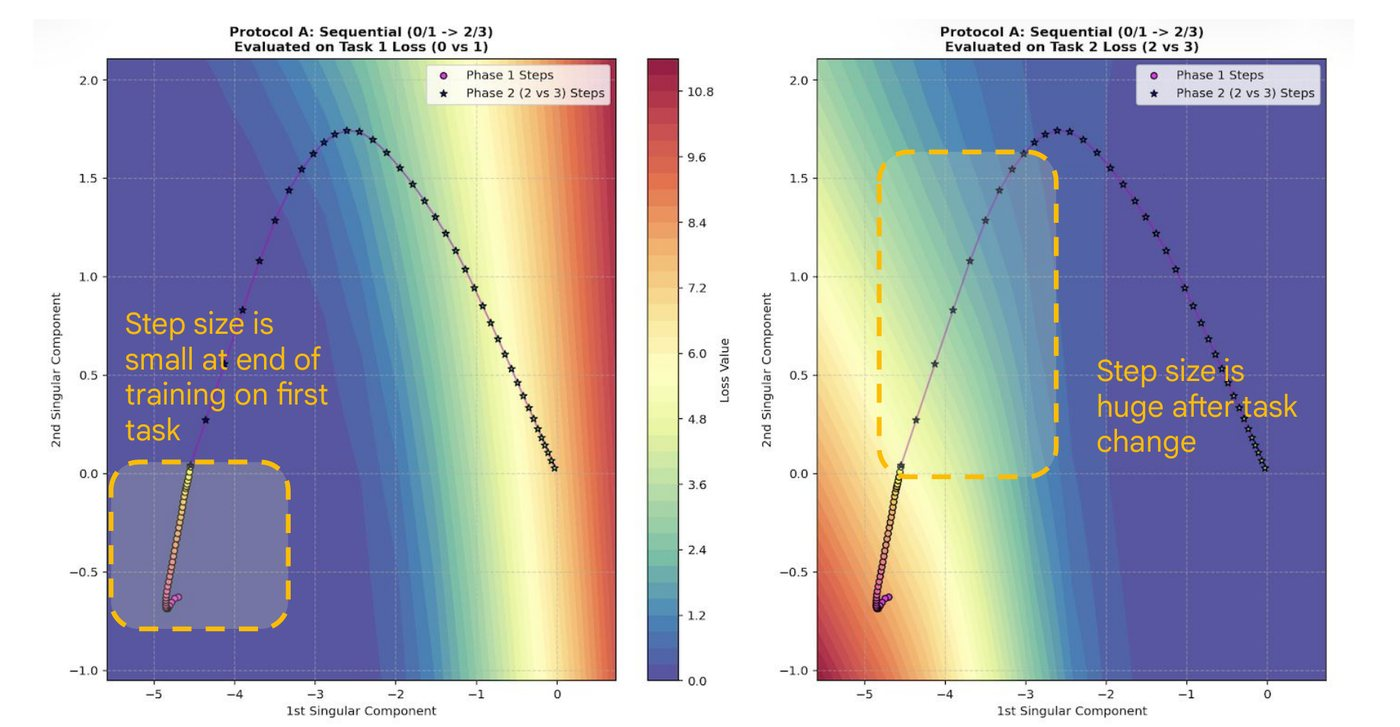
\includegraphics[width=0.90\textwidth]{figures/continual-learning-1.jpg}
\caption{Why plasticity is lost immediately rather than gradually, from the Continual Learning
lecture. The same optimisation trajectory is drawn over the task-one loss surface (left) and
the task-two loss surface (right), projected onto two singular components. Steps are tightly
packed at the end of task one, boxed on the left, and become very large as soon as the loss
switches to task two, boxed on the right. Adam's slow-decaying second moment still reflects
the small gradients of the previous task, so the effective step size overshoots.}
\label{fig:continual-learning-1}
\end{figure}

\paragraph{Why a large step is specifically destructive.} A large step does not merely
overshoot a minimum. It overshoots the receptive field of the nonlinearity: the preactivations
for a unit are pushed outside the range where the activation function is responsive, given the
feature covariance the network had built up. That is how ReLUs die. It also explains why the
remedy is not simply a smaller learning rate but control of the geometry, and it connects to a
neat observation in the lecture on parameter norm: rotating a large parameter vector by a given
angle requires a much larger perturbation than rotating a small one, so unchecked norm growth
makes the network progressively harder to move in function space
(Figure~\ref{fig:continual-learning-3}).

\begin{figure}[htbp]
\centering
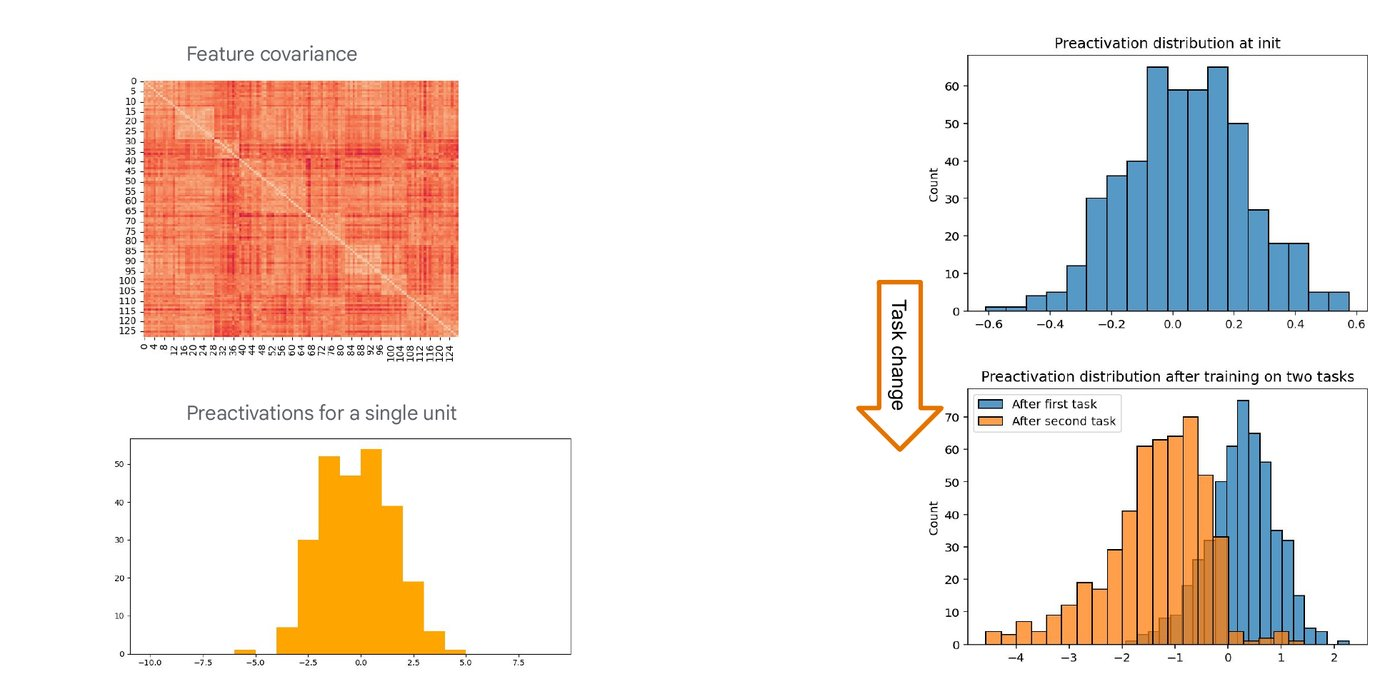
\includegraphics[width=0.90\textwidth]{figures/continual-learning-3.jpg}
\caption{How a large step kills a unit, from the Continual Learning lecture. Left, the feature
covariance the network has built up and the preactivation histogram for one unit. Right, the
same unit's preactivation distribution at initialisation, centred on zero and narrow, and after
training on two tasks: the second task's distribution, in orange, has shifted almost entirely
below zero. Once preactivations leave the range where the activation responds, the unit stops
passing gradient, which is what ``the ReLUs are dead'' means in practice.}
\label{fig:continual-learning-3}
\end{figure}

\paragraph{The fixes are boring.} What Lyle calls the swiss cheese approach
is three complementary interventions: control parameter norm growth, normalise preactivations,
and avoid regressing on ill-conditioned targets. The lesson is stated as use normalisation
layers and do not let parameters get too big. With these in place continual training stabilises
to the degree that the network can memorise effectively unlimited random labels of MNIST, and
the same treatment stabilises reinforcement learning. A separate and non-catastrophic route to
plasticity loss is warm-starting~\citep{ash2020}, tied to primacy bias: early in training a
model makes large changes relative to its current features, later only small ones. The proposed
remedy is to re-warm the effective learning rate above the threshold at which the model still
makes nontrivial changes to its features.

\section*{Notation}

The chapter follows the lecture's informal usage: $\task$ for a task, plasticity discussed
through the effective step size rather than a single symbol. Where the lecture refers to the
empirical NTK matrix it means the Gram matrix of per-example gradients at convergence, used as
a diagnostic of conditioning rather than as a theoretical object.

\section*{Why it matters}

This is the chapter that answers the closing slide of
Chapter~\ref{ch:01-intro-deep-learning}, where Chandar named non-i.i.d.\ learning as the
frontier without saying what breaks. The answer here is specific: the optimiser's state is
stale and the nonlinearity's receptive field is finite. It also stands in productive contrast
with Pascanu (Chapter~\ref{ch:07-to-be-figured-out}), who reaches for the same problem from
the direction of credit assignment and argues something stronger, that the i.i.d.\ assumption
is what makes gradient-based learning work at all. Lyle is the more optimistic of the two: her
position is that most plasticity loss is avoidable with best practices, and that resetting and
distilling remains available as a fallback.

\begin{aside}
The personal notes single out ``catastrophic forgetting'' as the takeaway and ask how to train
networks online. Lyle's answer, read carefully, is partly deflationary: where the data can be
stored, storing it is the right move, and the interesting problem only begins under a memory
constraint. Which regime a project is in decides whether the literature
applies at all, since it is largely written for the constrained case and most applications are
not.
\end{aside}
